\documentclass[12pt]{article}

\usepackage{multicol}
\usepackage{textcomp}
\usepackage{amsmath,amssymb,amsfonts,latexsym,stmaryrd,graphicx}
\usepackage[utf8]{inputenc}
\usepackage[T1]{fontenc}
\usepackage{xcolor}
\usepackage{anyfontsize}
\usepackage[spanish]{babel}
\usepackage{listings}
\usepackage{latexsym}
\usepackage[pdftex,breaklinks,colorlinks,linkcolor=black,citecolor=black,urlcolor=black]{hyperref}

\usepackage{epstopdf}
\DeclareGraphicsExtensions{.pdf,.png,.jpg,.gif,.eps}

\newcommand{\proof}{\textbf{Demostración:} }
\newcommand{\nl}{\vspace{0.3cm}}

\newtheorem{theorem}{Teorema}
\newtheorem{lemma}{Lema}
\newtheorem{definition}{Definición}
\newtheorem{corollary}{Corolario}

%opening
\title{Proyecto de Diseño y Análisis de Algoritmos\\ \vspace{.2cm} \textbf{Criba de Eratóstenes}}
\author{Leynier Gutiérrez González}

\begin{document}
	
\maketitle

\vspace{0.5cm}

\begin{center}
	\vspace{0.2cm}
	
\includegraphics[width=2.5cm]{images/escudo.png}\\
	\vspace{0.2cm}
	Facultad de Matemática y Computación\\
	\vspace{0.1cm}
	Universidad de La Habana\\
	\vspace{1cm}
\end{center}

\vspace{1cm}

\begin{abstract}
	En este documento haremos una breve introducción al algoritmo de la Criba de Eratóstenes. También veremos su complejidad temporal y espacial, así como, una variación de la misma Criba para poder calcular los primos menores que un $n$ dado muy grande, ahorrando memoria computando la Criba por segmentos. Luego mostraremos varias aplicaciones del algoritmo para resolver ejercicios.
\end{abstract}

\newpage

\tableofcontents

\newpage

\section{Criba de Eratóstenes}

\subsection{Introducción}

\nl

La Criba de Eratóstenes es un algoritmo simple para buscar todos los números primos menores que un número $n$.

\nl

La referencia más antigua conocida de la criba se encuentra en \textit{Introduction to Arithmetic}\cite{ngpia} de Nicomachus de Gerasa, que la describe y atribuye a Eratóstenes de Cyrene, un matemático griego.

\nl

Es una de las formas más eficientes de encontrar los números primos más pequeño y se puede utilizar para encontrar números primos en las progresiones aritméticas.\cite{eseapa}

\subsection{Descripción}

\nl

Se forma una tabla con todos los números naturales comprendidos entre $2$ y $n$, y se van tachando los números que no son primos de la siguiente manera: Comenzando por el $2$, se tachan todos sus múltiplos; comenzando de nuevo, cuando se encuentra un número entero que no ha sido tachado, ese número es declarado primo, y se procede a tachar todos sus múltiplos, así sucesivamente. El proceso termina cuando el cuadrado del siguiente número confirmado como primo es mayor que $n$.

\subsection{Implementación}

\lstinputlisting[language=Python]{codes/sieve.py}

\newpage

Este algoritmo produce todos los números primos que no son mayores que $n$. Incluye las optimizaciones comunes, que es comenzar a enumerar los múltiplos de cada $i$ primo desde $i^2$. La complejidad del tiempo de este algoritmo es $O(n \log(\log(n)))$\cite{aipns}, siempre que la actualización del array sea una operación $O(1)$, como suele ser el caso.

\nl

\subsection{Complejidad Temporal}

\nl

El trabajo realizado por este algoritmo es casi en su totalidad las operaciones para eliminar o marcar los números compuestos que, para la versión básica no optimizada es la suma del intervalo dividido por cada uno de los números primos hasta ese intervalo:

$$n \sum_{p \leqslant n}\frac{1}{p}$$

donde n es la longitud del intervalo de la criba en este y todos los análisis posteriores.

\nl

Al reorganizar el segundo teorema de Mertens, esto es igual a $n (\log(\log(n)) + M)$ a medida que $n$ se aproxima al infinito, donde $M$ es la constante de Meissel-Mertens.

\nl

La optimización de comenzar en el cuadrado de cada primo y solo seleccionar los primos menores que la raíz cuadrada cambia la $n$ en la expresión de arriba para $\sqrt{n}$ y no iterar hasta que el cuadrado significa que la suma de los primos base cada uno menos dos se resta de las operaciones. Como la suma de los primeros $x$ primos es $\frac{1}{2}x^2\log(x)$\cite{ant} y el teorema del número primo dice que $x \approxeq \frac{x}{\log(x)}$, donde la suma de los primos hasta $n$ es $\frac{n^2}{2 \log(n)}$, y por lo tanto la suma de los primeros primos hasta $\sqrt{n}$ es $\frac{1}{\log(n)}$ expresado como un factor de $n$. El intervalo entre dos primos es $2\pi(\sqrt{n})$, donde $\pi$ es la función para contar primos, o $\sqrt{4\sqrt{n}}$, expresando esto como un factor de $n$ como lo son los otros términos, esto es $\frac{4}{\sqrt{n}\log(n)}$. Combinando todo esto, la expresión para el número de operaciones con las optimizaciones sin la factorización de la rueda es:

$$\log(\log(n)) - \frac{1}{\log(n)} \left(1  -\frac{4}{\sqrt{n}}\right) + M - \log(2)$$

Para los casos de factorización de ruedas, hay un desplazamiento adicional de las operaciones no realizadas de:

$$ \sum_{p \leqslant x}\frac{1}{p} $$

donde $x$ es el número primo más alto de la rueda y se aplica un factor constante de toda la expresión que es la fracción de los candidatos primarios restantes en comparación con la circunferencia de la rueda que se repite. La circunferencia de la rueda es:

$$ \prod_{p \leqslant x}p $$

y se puede determinar fácilmente que este factor de rueda es:

$$ \prod_{p \leqslant x}\frac{p - 1}{p} $$

como $\frac{p - 1}{p}$ es la fracción de los candidatos restantes para el primo de rueda más alto, $x$, y cada primo menor subsiguiente deja su fracción correspondiente de la fracción combinada anterior.

\nl

Combinando todo el análisis anterior, el número total de operaciones para una criba hasta $n$, incluida la factorización de la rueda para primos hasta $x$, es aproximadamente:

$$ \prod_{p \leqslant x}\frac{p - 1}{p} \left( \log(\log(n)) - \frac{1}{\log(n)} \left(1  -\frac{4}{\sqrt{n}}\right) + M - \log(2) - \sum_{p \leqslant x}\frac{1}{p} \right) $$

Para mostrar que la expresión anterior es una buena aproximación al número de operaciones para eliminar los números compuestos realizadas por el algoritmo, a continuación se muestra una tabla que muestra el número de operaciones realmente medido para una implementación práctica de la criba de Eratóstenes en comparación con el número de operaciones que se predice a partir de la expresión anterior, tanto expresados como una fracción del intervalo (redondeado a cuatro lugares decimales) para diferentes intervalos de la criba y factorizaciones de rueda (tenga en cuenta que la última columna es una rueda práctica máxima en cuanto al tamaño de los huecos de las ruedas) - casi 10 millones de valores):

\begin{center}
	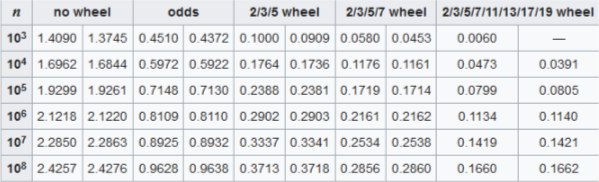
\includegraphics[width=10cm]{images/table1.png}
\end{center}

La tabla anterior muestra que la expresión anterior es una muy buena aproximación al número total de operaciones de la criba de alrededor de cien mil (105) y superiores.

\nl

La criba de Eratóstenes es una forma popular de comparar el rendimiento de las computadoras. \cite{ompts} Como se puede ver de lo anterior al eliminar todas las operaciones constantes y los factores constantes e ignorar los términos que tienden a cero a medida que $n$ se acerca al infinito, la complejidad temporal para calcular todos los primos menores que $n$ en el modelo de máquina de acceso aleatorio es $O(n\log(\log(n)))$ operaciones, una consecuencia directa del hecho de que la serie armónica principal se aproxima asintóticamente a $\log(\log(n))$. Sin embargo, tiene una complejidad de tiempo exponencial con respecto al tamaño de entrada, lo que lo convierte en un algoritmo pseudo-polinómico. El algoritmo básico requiere $O(n)$ de memoria.

\nl

La complejidad basada en bits del algoritmo es $O(n(\log(n)) (\log(\log(n))))$ operaciones de bit con un requisito de memoria de $O(n)$.\cite{lpnsaft}

\section{Criba Segmentada}

\subsection{Introducción}

\nl

Como señala Jon Sorenson, el problema con la criba de Eratóstenes no es el número de operaciones que realiza, sino sus requisitos de memoria.\cite{aipns} Para $n$ grande, el intervalo de números primos puede no caber en la memoria. Peor aún, incluso para $n$ no tan grandes, su uso de caché es altamente subóptimo. El algoritmo recorre todo el array, sin mostrar casi ninguna localidad de referencia.

\newpage

Las cribas segmentadas ofrecen una solución a estos problemas, donde solo se computa partes del intervalo a la vez.\cite{pnap} Se conocen desde la década de 1970 y funcionan de la siguiente manera:\cite{aipns}\cite{ssepap}

\subsection{Descripción}

\nl

La idea de una criba segmentada es dividir el intervalo $[0 .. n-1]$ en diferentes segmentos y calcular los primos en todos los segmentos uno por uno. Este algoritmo primero usa la criba común para encontrar números primos más pequeños o iguales a $\sqrt{n}$. A continuación se presentan los pasos utilizados en la criba segmentada.\cite{gfgss}

\begin{enumerate}
	\item Use una criba común para encontrar todos los números primos hasta $\sqrt{n}$ y almacene estos números primos en una lista.
	\item Necesitamos todos los números primos en el intervalo $[0..n-1]$. Dividimos este intervalo en diferentes segmentos, de manera que el tamaño de cada segmento es como máximo $\sqrt{n}$.
	\item Hacer lo siguiente para cada segmento $[comienzo ... final]$.
	\begin{itemize}
		\item Crear un array de tamaño $final - comienzo + 1$. Aquí solo necesitamos $O(x)$ espacio donde $x$ es el número de elementos en un intervalo dado.
		\item Iterar a través de todos los números primos encontrados en el paso $1$. Para cada número primo, marque sus múltiplos en el intervalo dado $[comienzo ... final]$.
	\end{itemize}
\end{enumerate}

\subsection{Complejidad Temporal}

\nl

La versión de la criba segmentada tiene la misma complejidad temporal de $O(n \log(\log(n)))$ que la versión común, pero reduce la complejidad espacial al tamaño mínimo de la longitud del segmento más la memoria requerida para almacenar los números primos base menores que la raíz cuadrada de la longitud del segmento utilizado para marcar y eliminar los compuestos de los segmentos sucesivos $O\left(\frac{\sqrt{n}}{\log(n)}\right)$.

\subsection{Implementación}

\lstinputlisting[language=Python]{codes/segmented_sieve.py}

\section{Problemas}

\subsection{Números casi primos}

\nl

\subsubsection{Descripción}

Los números casi primos son los números no primos que son divisibles por un solo número primo. En este problema, su trabajo consiste en escribir un programa que encuentre la cantidad de números casi primos dentro de un cierto intervalo.

\nl

\textbf{Entrada:} La primera línea del archivo de entrada contiene un entero $N (N \leqslant 600)$ que indica cuántos conjuntos de entradas hay. Cada una de las siguientes $N$ líneas hace un único conjunto de entrada. Cada conjunto contiene dos números enteros $bajo$ y $alto$ $(0 < bajo \leqslant alto < 10^{12})$.

\nl

\textbf{Salida:} Para cada línea de entrada, excepto la primera línea, debe producir una línea de salida. Esta línea contiene un solo entero, que indica cuántos números casi primos están dentro del intervalo (inclusivo) $[bajo ... alto]$.

\nl

\textbf{Ejemplo de Entrada:}

\nl

\begin{tabular}{|l|l|}
	\hline 3 &  \\ 
	\hline 1 & 10 \\ 
	\hline 1 & 20 \\ 
	\hline 1 & 5 \\ 
	\hline 
\end{tabular} 

\nl

\textbf{Ejemplo de Salida:}

\nl

\begin{tabular}{|c|}
	\hline 3 \\ 
	\hline 4 \\ 
	\hline 1 \\ 
	\hline 
\end{tabular} 

\nl

\subsubsection{Solución}

\textbf{Primera idea fallida:} Utilizar un array de $int$ inicializados en $0$ en vez de un array de $bool$. Los primos quedarían con el valor $0$ y para los compuestos en vez de marcarlos como $false$, aumentar el valor en el array. Al final del proceso de la criba quedaría en el array para la posición i-ésima la cantidad de divisores primos del número $i$ a menos que $i$ sea primo que en este caso sería el valor $0$. Luego hacer una tabla acumulativa con los valores del array iguales a $1$ ya que estos son los únicos números divisibles por un único primo y que no son primos. El problema que tiene esta idea es que el intervalo es hasta $10^{12}$ y necesitariamos un array de esta longitud, lo cual no es posible.

\nl

\textbf{Idea correcta:} Calcular los primos hasta $10^6$ y guardarlos en una lista. Luego en esta lista ir haciendo búsquedas binarias para los valores de las raíces del límite inferior y superior e ir acumulando la diferencia del resultado de las búsquedas hasta que la raíz del límite superior sea menor que $2$.

\nl

\textbf{Demostración:}

\begin{theorem}
	$x$ es casi primo $\iff$ $\exists$ $k \in \mathbb{Z^*}\ k > 1$ y $p \in primos$ tal que $p^k = x$.
\end{theorem}

\newpage

\proof Si $x$ es casi primo entonces es divisible por un único primo. Luego, por el teorema fundamental de la Aritmética $x = p^k$ y como $x$ no es primo, por ser casi primo, necesariamente $k > 1$. Por otro lado, si existen $p$ y $k$ tal que se cumplan las condiciones del lado derecho entonces por el teorema fundamental de la Aritmética $p$ y $k$ son únicos, dando lugar a que $x$ no sea primo y sea divisible por un único primo.

\begin{theorem}
	Buscar la cantidad de potencias k-ésimas de números primos entre $a$ y $b$ es lo mismo que buscar la cantidad de primos entre $\sqrt[k]{a}$ y $\sqrt[k]{b}$.
\end{theorem}

\proof Es consecuencia de que $\sqrt[k]{a} \leqslant p \leqslant \sqrt[k]{b} \Rightarrow a \leqslant p^k \leqslant b$.

\nl

\textbf{Código:} \href{https://gist.github.com/leynier/99a2f30059f118f1d8afd59489b4ebd9}{gist.github.com/leynier/99a2f30059f118f1d8afd59489b4ebd9}

\nl

\textbf{Fuente:} \href{http://coj.uci.cu/24h/problem.xhtml?pid=1938}{coj.uci.cu/24h/problem.xhtml?pid=1938}

\subsection{Doble felicidad}

\subsubsection{Descripción}

En la lección de matemáticas, un profesor le pidió a cada alumno que sacara sus propios números de la suerte. Como fanático de la teoría de números, Peter eligió los números primos. Bob era más original. Dijo que el número $t$ es su número de la suerte, si se puede representar como:

$$ t = a^2 + b^2 $$

donde $a$ y $b$ son enteros positivos arbitrarios.

\nl

Ahora, los niños decidieron averiguar cuántos días del intervalo $[l, r]$ $(l \leqslant r)$ son adecuados para la programación de pares. Decidieron que el día $i$ $(l \leqslant i \leqslant)$ es adecuado para la programación de pares si y sólo si el número $i$ es afortunado para Peter y para Bob al mismo tiempo. Ayuda a los chicos a encontrar el número de esos días.

\nl

\textbf{Entrada:} La primera línea de la entrada contiene los números enteros $l, r$ $(1 \leqslant l, r \leqslant 3 * 10^8)$.

\nl

\textbf{Salida:} En la única línea, imprima el número de días en el segmento $[l, r]$, que son afortunados para Peter y Bob al mismo tiempo.

\newpage

\textbf{Ejemplo de Entrada 1:} $3 5$

\nl

\textbf{Ejemplo de Salida 1:} $1$

\nl

\textbf{Ejemplo de Entrada 2:} $6\ 66$

\nl

\textbf{Ejemplo de Salida 2:} $7$

\nl

\subsubsection{Solución}

La solución pasa por utilizar el teorema de Fermat\cite{oftst} que dice que un número primo $p$ es expresable como suma de dos cuadrados si y sólo si $p = 2$ ó $p \equiv 1 (mod\ 4)$.

\nl

Luego solo basta con buscar los primos en el intervalo y contar los que dejen resto $1$ al ser divididos por $4$.

\nl

Importante notar que el intervalo es muy grande, por lo que se hace necesario utilizar una criba segmentada para resolver el problema.

\nl

\textbf{Código:} \href{https://gist.github.com/leynier/937401c77149a6fe02781218d78ce5dd}{gist.github.com/leynier/937401c77149a6fe02781218d78ce5dd}

\nl

\textbf{Fuente:} \href{https://codeforces.com/contest/114/problem/E}{codeforces.com/contest/114/problem/E}

\subsection{Mi niña bonita Noora}

\subsubsection{Descripción}

En la Universidad de Pavlopolis, donde estudia Noora, se decidió celebrar el concurso de belleza \textit{Universidad Miss Pavlopolis}. Vamos a describir el proceso de elegir a la chica más hermosa de la universidad con más detalle.

\nl

El concurso se lleva a cabo en varias etapas. Supongamos que exactamente $n$ chicas participan en la competencia inicialmente. Todos los participantes se dividen en grupos iguales, $x$ cantidad de participantes en cada grupo. Además, el número $x$ se elige arbitrariamente, es decir, en cada etapa el número $x$ puede ser diferente. Dentro de cada grupo, el jurado del concurso compara la belleza de las chicas en el formato \textit{todas contra todas}. De esta manera, si el grupo consiste en $x$ niñas, entonces se producen $\frac{x(x-1)}{2}$ comparaciones. Luego, de cada grupo, se selecciona el participante más bello. Las chicas seleccionadas ingresan a la siguiente etapa del concurso. Por lo tanto, si $n$ niñas se dividieron en grupos, $x$ cantidad de participantes en cada grupo, entonces exactamente $\frac{n}{x}$ participantes ingresarán a la siguiente etapa. El concurso continúa hasta que quede exactamente una niña que será \textit{Miss Pavlopolis University}.

\nl

Pero para el jurado este concurso es una tarea muy tediosa. Les gustaría dividir a las niñas en grupos en cada etapa para que el número total de comparaciones por parejas de las niñas sea lo menos posible. Sea $f(n)$ el número total mínimo de comparaciones que deben realizarse para seleccionar al participante más hermoso, si admitimos $n$ chicas en la primera etapa.

\nl

Los organizadores del concurso están locos. Le dan a Noora tres enteros $t$, $l$ y $r$, y le piden a la pobre chica que calcule el valor de la siguiente expresión:

$$ t^0 * f(l) + t^1 * f(l + 1) + ... + t^{r - l} * f(r) $$

\nl

Sin embargo, dado que el valor de esta expresión puede ser bastante grande, los organizadores le piden que la calcule módulo $10^9 + 7$. Si Noora puede calcular el valor de esta expresión, los organizadores le prometen ayuda durante el concurso de belleza. Pero la pobre niña no es fuerte en matemáticas, así que buscó ayuda con Leha y él se dirigió a ti.

\nl

\textbf{Entrada:} La primera y única línea contiene tres enteros $t$, $l$ y $r$ $(1 \leqslant t < 10^9 + 7,\ 2 \leqslant l \leqslant r \leqslant 5 * 10^6)$.

\nl

\textbf{Salida:} En la primera línea, imprimir un solo entero: el valor de la expresión módulo $10^9 + 7$.

\nl

\textbf{Ejemplo de Entrada:} $2\ 2\ 4$

\nl

\textbf{Ejemplo de Salida:} $19$

\subsubsection{Solución}

Supongamos que ya hemos calculado $f(2)$, $f(3)$, $...$, $f(r)$. Entonces, calcular el valor de la expresión es fácil.

\nl

Consideremos el proceso de cálculo de $f(x)$. Supongamos que encontramos una respuesta óptima. Representemos esta respuesta como una secuencia de números enteros $d_1, d_2, ..., d_k$: en la primera etapa dividiremos a las niñas en grupos de participantes de $d_1$, en la segunda etapa en grupos de participantes de $d_2$ y así sucesivamente. Probemos que todos los $d_i$ deben ser primos.

\nl

Supongamos que algún $d_i$ es un número compuesto. Luego lo podemos descomponer en dos números $d_i = a * b$. Además, sea $n$ el número de chicas que son admitidas en la i-ésima etapa. Luego en la actual i-ésima etapa ocurrirán $ \frac{n}{d_i} * \frac{d_i(d_i - 1)}{2} =  \frac{n(d_i - 1)}{2}$ comparaciones. Pero si dividimos esta etapa en dos nuevas etapas, entonces el número de comparaciones es $ \frac{n(a-1)}{2} + \frac{n(b - 1)}{2a} \leqslant \frac{n(a-1)}{2} + \frac{n(b-1)}{2} \leqslant \frac{n(a+b-2)}{2} \leqslant \frac{n(ab - 1)}{2} = \frac{n(d_i - 1)}{2}$. Por lo tanto, hemos demostrado que todos los $d_i$ deben ser primos. Entonces es fácil escribir una dinámica, que se calculará mediante la transición del estado a los estados dados al dividir el estado actual entre los divisores primos. Para resolver esta tarea podemos utilizar la criba de Eratóstenes.

\nl

\textbf{Código:} \href{https://gist.github.com/leynier/b79194f3397e3ac546aa01cf2c408462}{gist.github.com/leynier/b79194f3397e3ac546aa01cf2c408462}

\nl

\textbf{Fuente:} \href{https://codeforces.com/contest/822/problem/D}{codeforces.com/contest/822/problem/D}

\newpage

\nocite{*}
\bibliographystyle{unsrt}
\bibliography{sieve}
	
\end{document}
